%#! latexmk -pv IAB_DYNAMICO_kernels
\section{\src{comp_pvort}}

\subsection{Description}

Kernel \src{comp_pvort} is taken from the original subroutine
\src{compute_pvort} in \DYNAMICO.
%
This subroutine is originally defined in module \src{caldyn_gcm_mod}.
%
This module defines subroutine \src{caldyn}, which is the main
subroutines for dynamics part of the model, and several sub-subroutines
for various terms in the governing equation, such as potential
vorticity, geopotential, etc.
%
This subroutine calculates potential vorticity.


\subsection{Discretization and code}

\autoref{l:definition_comp_pvort} shows the definition part of this subroutine
and \autoref{f:pad_comp_pvort} shows the PAD of
this.
%
Note that sources shown here are modified in the process of
kernelization from the original distributed version.

\begin{LstF90}[%
caption={Definition part of \src{compute_pvort}},%
label={l:definition_comp_pvort}%
]
SUBROUTINE compute_pvort(ps,u,theta_rhodz, rhodz,theta,qu,qv)
  USE icosa
  USE disvert_mod, ONLY : mass_dak, mass_dbk, caldyn_eta, eta_mass
  USE exner_mod
  USE trace
  USE omp_para
  IMPLICIT NONE
  REAL(rstd),INTENT(IN)  :: u(iim*3*jjm,llm)
  REAL(rstd),INTENT(IN)  :: ps(iim*jjm)
  REAL(rstd),INTENT(IN)  :: theta_rhodz(iim*jjm,llm)
  REAL(rstd),INTENT(INOUT) :: rhodz(iim*jjm,llm)
  REAL(rstd),INTENT(INOUT) :: theta(iim*jjm,llm)
  REAL(rstd),INTENT(INOUT) :: qu(iim*3*jjm,llm)
  REAL(rstd),INTENT(INOUT) :: qv(iim*2*jjm,llm)

  INTEGER :: i,j,ij,l
  REAL(rstd) :: etav,hv, m
\end{LstF90}
%
Here \src{u}, \src{ps}, \src{theta_rhodz} are velocity on the edge, surface pressure,
and mass-weighted potential temperature, respectively.
Output arrays \src{rhodz}, \src{theta}, \src{qu}, \src{qv} are mass, potential temperature,
potential vorticity on the edge, and potential vorticity on the vertex, respectively.
%
These arrays except \src{ps} have two dimensions, first one is for
horizontal index and second one is for vertical index.
%
Note that \DYNAMICO adopts C-grid in horizontal, number of horizontal
grid point for scalar, or number of control volume, in one domain is
\src{iim*jjm}, but \src{u} and \src{qu} are defined on the edge of
control volume, the size of the first dimension of them are
\src{iim*3*jjm}.  Also \src{qv} is defined on the vertex of control
volume, the size of the first dimension of \src{qv} is \src{iim*2*jjm}.

\begin{figure}[htbp]
 \centering
 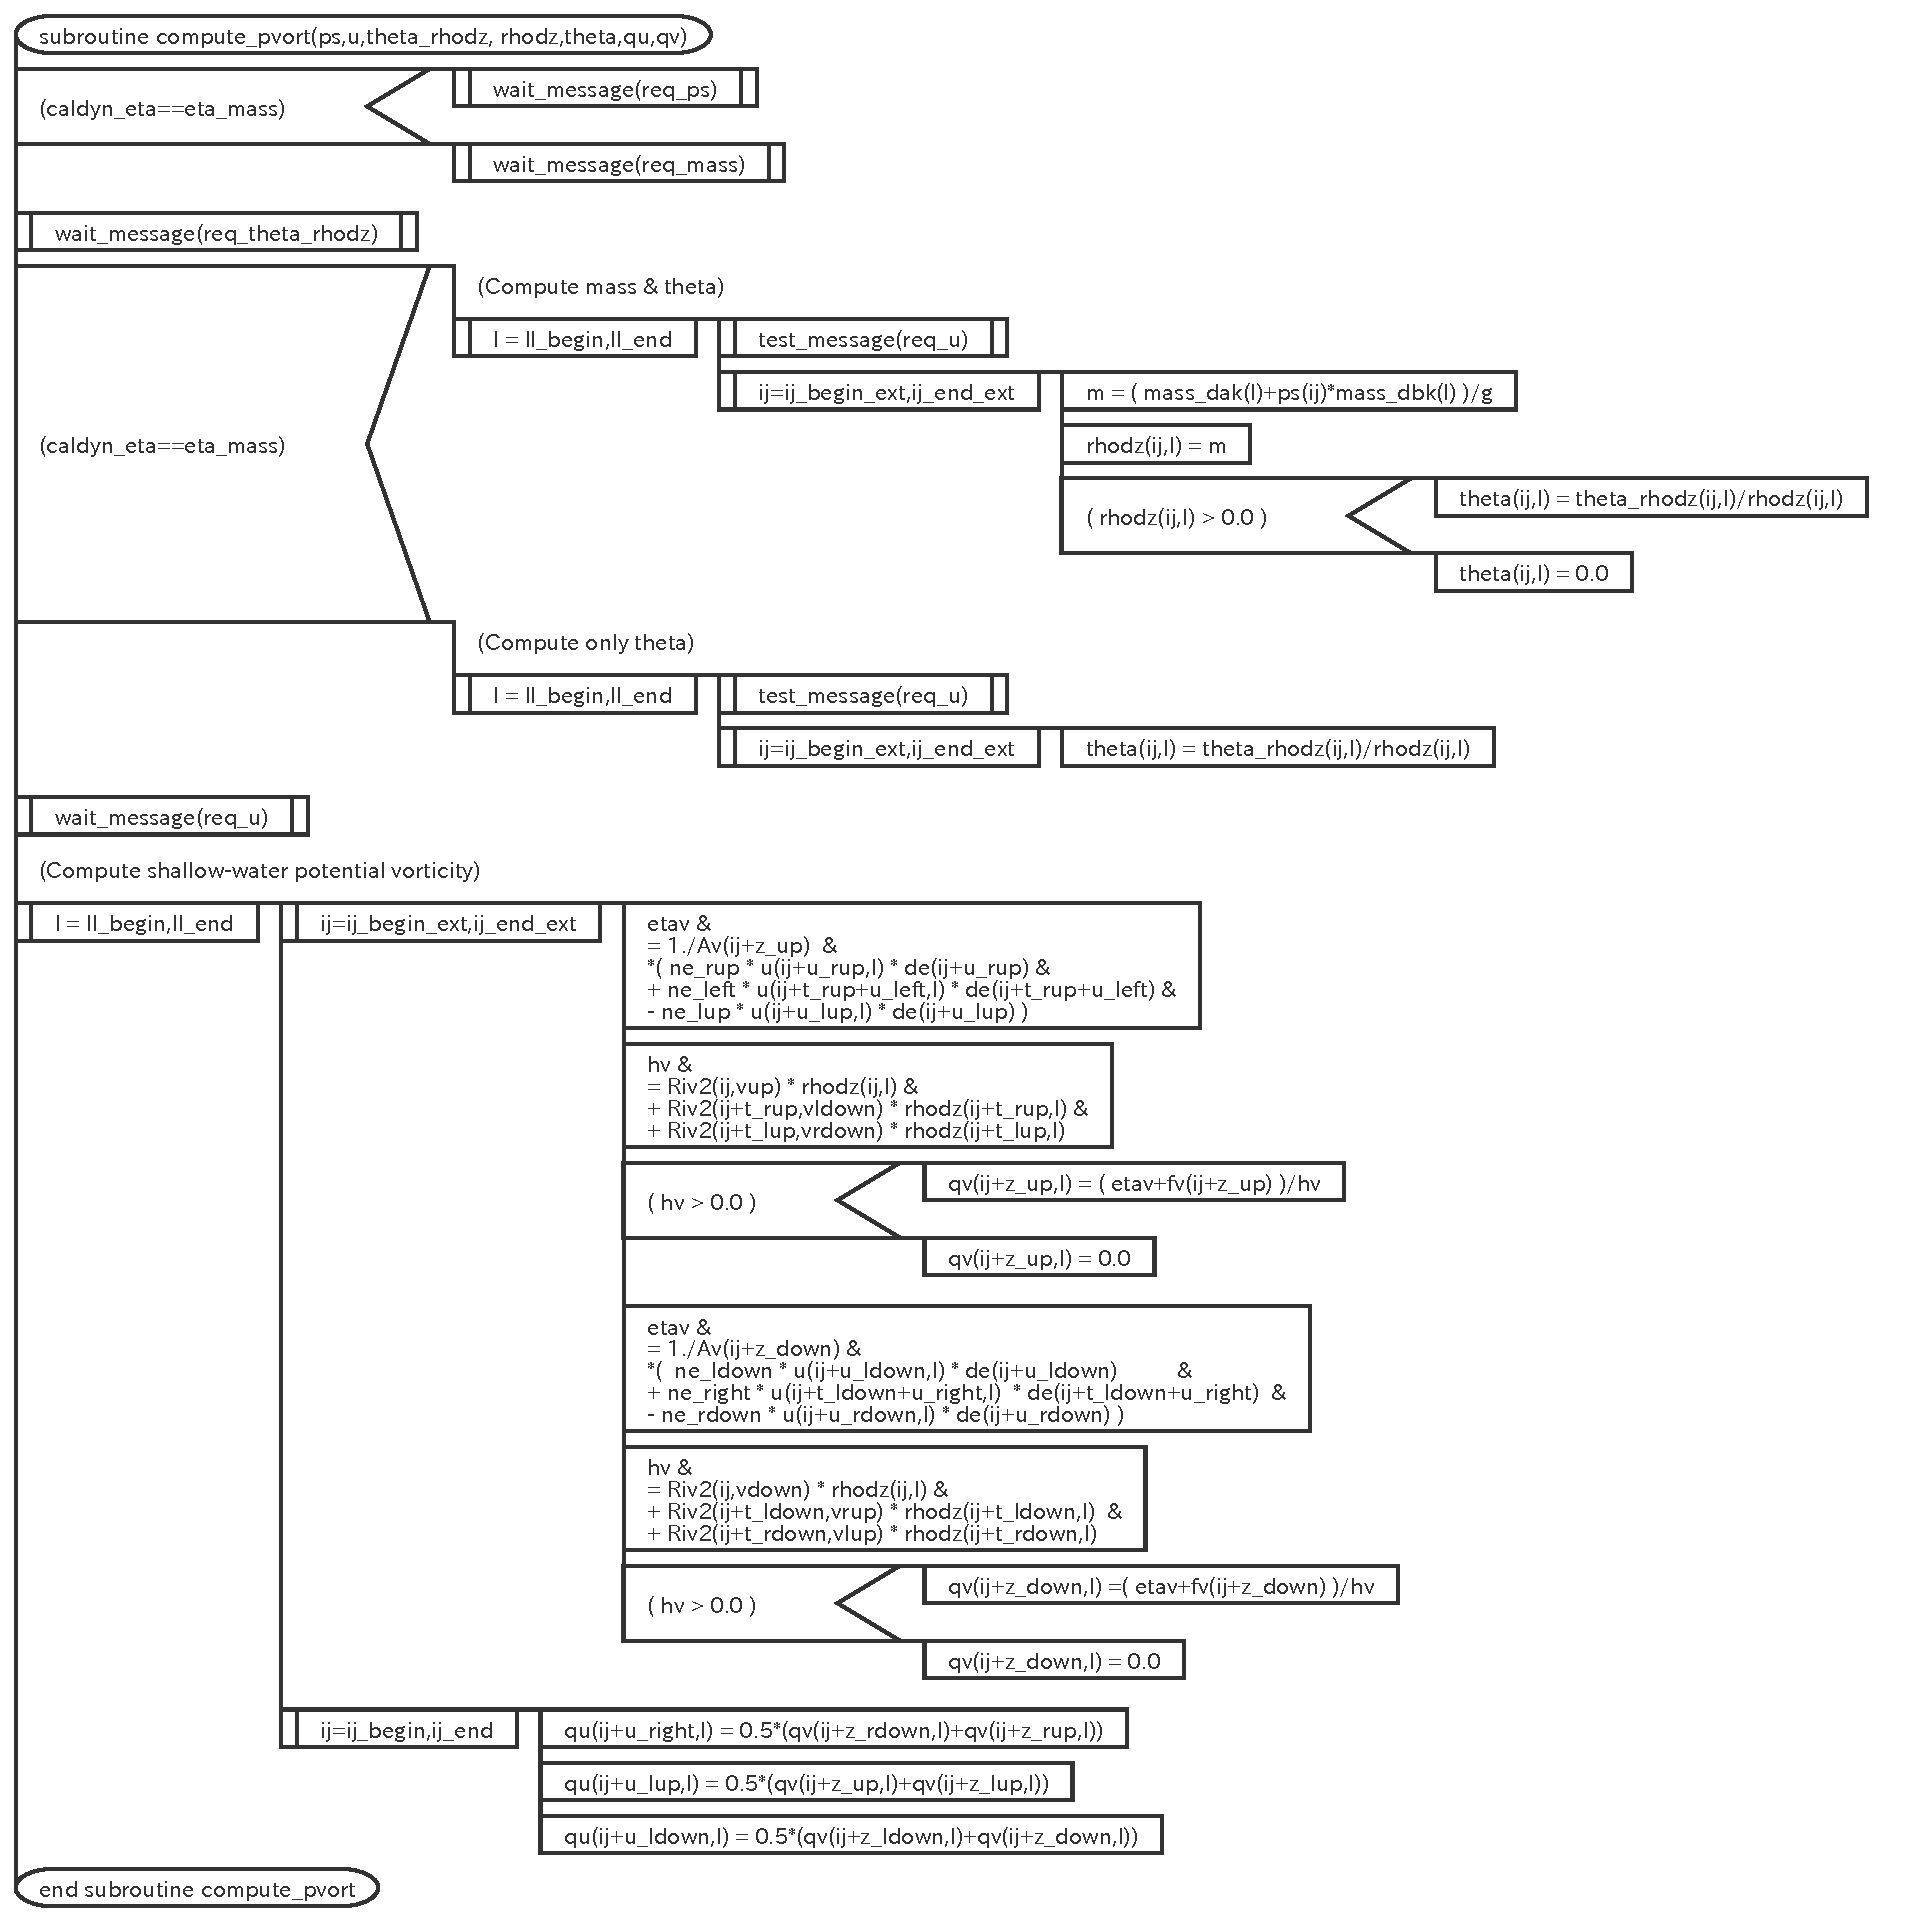
\includegraphics[scale=.4]{figs/pvort.pdf}
 \caption{PAD of \src{compute_pvort}}\label{f:pad_comp_pvort}%
\end{figure}

The first section of this subroutine calculates \src{theta} in the
double loop of \src{ij} and \src{l}.
%
Note that in this kernel package, \src{caldyn_eta} is set as
\src{eta_mass}, that means that vertical coordinate $\eta$ uses
Lagrangian vertical coordinate, rather than mass coordinate.
%
In the second section, \src{qv} at two points, \src{qv(ij+z_up,l)} and
\src{qv(ij+z_down,l)}, are calculated in the first double loop, then
\src{qu} at three pounts, \src{qu(ij+u_right,l)}, \src{qu(ij+u_lup,l)}
and \src{qu(ij+l_down,l)} are calculated.

\clearpage



\subsection{Input data and result}

Input data file is prepared and you can download from official server using
\file{data/download.sh} script.
%
This data file is created by original \DYNAMICO\footnotemark with
Held-Suarez case parameter set included in the original source archive.
%
\footnotetext{with slight modification by AICS.}
%
Max/min/sum of input/output data of the kernel subroutine are output as
a log.
%
Below is an example of \src{$IAB_SYS=Ubuntu-gnu-ompi} case.

\begin{LstLog}
 [KERNEL] comp_pvort
 *** Start  initialize
                iim, jjm, llm:    23    25    19
             ij_begin, ij_end:    48   528
     ij_begin_ext, ij_end_ext:    24   552
             ll_begin, ll_end:     1    19
        t_right, t_rup, t_lup:     1    23    22
     t_left, t_ldown, t_rdown:    -1   -23   -22
        u_right, u_rup, u_lup:     0  1173   575
     u_left, u_ldown, u_rdown:    -1  1150   553
           z_rup, z_up, z_lup:   598     0   597
     z_ldown, z_down, z_rdown:   -23   575   -22
                   caldyn_eta:     1
                            g:     9.80000000
 +check[Av              ] max=  4.1228713627140027E+11,min=  0.0000000000000000E+00,sum=  3.2428753277257527E+13
 +check[de              ] max=  4.5171816240714993E+06,min=  0.0000000000000000E+00,sum=  4.7785815753077912E+08
 +check[Riv2            ] max=  3.8193271158709069E-01,min=  0.0000000000000000E+00,sum=  9.6499999999999977E+02
 +check[fv              ] max=  8.2383275804860789E-05,min= -6.6879410680009186E-05,sum=  4.1115175112148659E-03
 +check[mass_dak        ] max=  3.9864758943842335E+03,min= -4.2200064724847380E+03,sum=  1.1368683772161603E-13
 +check[mass_dbk        ] max=  1.6280745944237918E-01,min=  0.0000000000000000E+00,sum=  1.0000000000000000E+00
 *** Finish initialize
 *** Start kernel
 ### check point iteration:        1000
 ### Input ###
 +check[u               ] max=  4.1278968179782127E-01,min= -4.1278968179782127E-01,sum=  1.6791131703073393E+01
 +check[ps              ] max=  1.0000000000000000E+05,min=  1.0000000000000000E+05,sum=  5.7500000000000000E+07
 +check[theta_rhodz     ] max=  3.9393370687019045E+05,min=  0.0000000000000000E+00,sum=  1.8099621340626464E+09
 +check[theta_prev      ] max=  8.0139914420291746E+02,min=  0.0000000000000000E+00,sum=  3.8582633571973117E+06
 +check[rhodz_prev      ] max=  1.2306877011993038E+03,min=  0.0000000000000000E+00,sum=  5.3979591836733194E+06
 +check[qu_prev         ] max=  1.0339537867296609E-06,min= -8.4408169682701225E-07,sum=  3.9419811615778674E-04
 +check[qv_prev         ] max=  1.0397552030841796E-06,min= -8.4408169685381862E-07,sum=  2.6984926372303133E-04
 ### Output ###
 +check[theta           ] max=  8.0139914420291746E+02,min=  0.0000000000000000E+00,sum=  3.8582633571973117E+06
 +check[rhodz           ] max=  1.2306877011993038E+03,min=  0.0000000000000000E+00,sum=  5.3979591836733194E+06
 +check[qu              ] max=  1.0626772908333491E-06,min= -8.5290650439776975E-07,sum=  3.9864842567446446E-04
 +check[qv              ] max=  1.0855993800007362E-06,min= -8.9078811385791910E-07,sum=  2.7461310165802981E-04
 ### final iteration:        1000
 ### Validation : grid-by-grid diff ###
 +check[theta           ] max=  0.0000000000000000E+00,min=  0.0000000000000000E+00,sum=  0.0000000000000000E+00
 +check[rhodz           ] max=  0.0000000000000000E+00,min=  0.0000000000000000E+00,sum=  0.0000000000000000E+00
 +check[qu              ] max=  0.0000000000000000E+00,min=  0.0000000000000000E+00,sum=  0.0000000000000000E+00
 +check[qv              ] max=  0.0000000000000000E+00,min=  0.0000000000000000E+00,sum=  0.0000000000000000E+00
 *** Finish kernel
\end{LstLog}

Check the lines below \src{``Validation : grid-by-grid diff''} line,
that shows difference between calculated output array and
pre-calculated reference array.
These should be zero or enough small to be acceptable.
%
There are sample output log files in \file{reference/}
in each kernel program directory, for reference purpose.


\subsection{Sample of performance result}

Here's an example of the performance result part of the log output.
Below is an example executed with the machine environment described in \autoref{s:measuring_env}.
%
Note that in this program kernel part is iterated 1000 times.

\begin{LstLog}
 *** Computational Time Report
 *** ID=001 : MAIN_comp_pvort                  T=     0.248 N=   1000
\end{LstLog}
